\chapter{PLACEMENT OF FIGURES IN \LaTeX }\label{chap2:body1}


When creating figures in \LaTeX, it is important to realize that
different types of figures are imported differently, leading to
different margins below the figure.
For diagrams, as in Figure~\ref{pg1},
\TeX CAD (see \cite{texcad}) is recommended since it creates
native vector images, and text in it will match the rest of your project.
The line in Figure~\ref{pg1} is at height $y=0$ in \TeX CAD.
The distance between the figure and the caption is supposed to be
a double space.
Hence your lowest object should be at height $y=???$mm in \TeX CAD.
A double space should separate the figure from paragraph text
above or below it, which is done in Figure \ref{pg1}.

\begin{figure}[htb]
\centering
\input{figs/petersen_graph_with_bottom.pic}
\caption{
The line in the figure above is at height $y=0$ in \TeX CAD.
Note that \LaTeX \ automatically typesets captions single-spaced.
}
\label{pg1}
\end{figure}

There will be more white space between the ``bottom" of the figure and
the caption if the lowest object is higher than $y=0$.
Figure \ref{pg3} shows how items that are placed too high can
distort the distance between the image and the caption.
I've configured the float spacing to get appropriate results
--- doublespace between the float and surrounding paragraphs --- but
if it gives you trouble then use \verb+\vspace{}+ to add or subtract
vertical space.

\begin{figure}[htb]
\centering
\input{figs/petersen_graph_high.pic}
\caption{If your figure has some white space above the unseen actual border,
like this one, only less extreme, please make a note on the printout that
goes to the proofreader. Without the line on the bottom and the text,
this figure would not be acceptable (too much white space).
Disclaimer: This is an example of a {\bf bad} figure with too much
white space between content and bounding box.}
\label{pg3}

\end{figure}



Because \LaTeX \ treats figures as floating objects,
the correct placement of figures is effected with the
\verb+[htb]+ (``here, top, or bottom") option.
Placing your figure after the paragraph that first refers to it
and using \verb+[hbt]+ will place the figure right there, if possible, and,
if not, it will place the figure at bottom of the page, or
the top of the next page,
which is in accordance with technical writing rules.
This is how Figures \ref{pg1} and \ref{pg3} were placed.

Most picture formats can be imported. In Figure~\ref{batgull2},
the default distance between the bottom of the picture and the
caption is different than when a picture environment was imported
and the distance was corrected with the \verb+\vspace+ command.



\begin{figure}[hbt] %% figure
\begin{center}
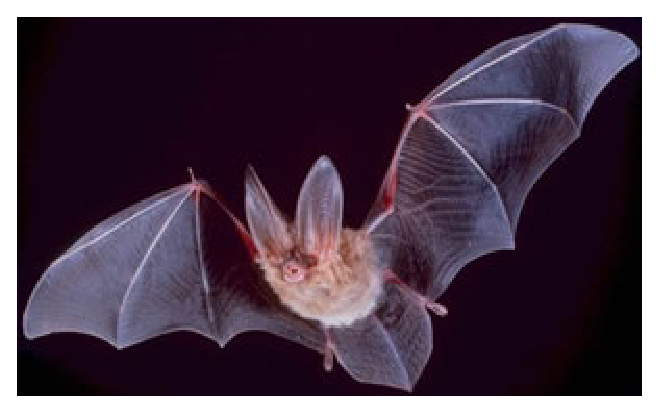
\includegraphics[width=.45\linewidth]{figs/bat_b.eps}\hspace*{0.04in}
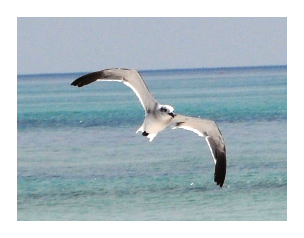
\includegraphics[width=.36\linewidth]{figs/gull2_b.eps}\\
\end{center}
\vspace{-.1in}

\caption
{
Note how a picture that was created or imported differently has a different
space between caption and image than the line drawing in Figure
\protect\ref{pg1}. (Left) Bat flight is being studied as part of an
Air Force Office of Scientific Research Multidisciplinary
University Research Initiative project.
Image credit: mime.oregonstate.edu/news/story/2103, (Right)
Morphing gull wings.
{\em Note how the URL spills too far to the right in the
list of figures. This type of margin infraction must be
corrected manually.}}
\label{batgull2}
\end{figure}



Note that imported pictures that have white space on their margins
will look
as if they are placed incorrectly. For such pictures,
make a note on the printout that goes to format checking.



\section{Tables}

Tables pretty much act like figures. Table~\ref{tablelabel}
is an example of a small table.


\begin{table}[h]
\cprotect\caption{A sample table. If there are no tables,
comment out the \verb+% this contains:
% list of tables
%DO NOT CHANGE IT.





\newpage

% lists of figures and tables
\addcontentsline{toc}{chapter}{LIST OF TABLES}
\begin{singlespace}

%%%\singlespacing
% This configures the space before the title
\renewcommand{\cftbeforelottitleskip}{.6in}%{\SpaceBeforeChapter}
% this configures the space after the title
\renewcommand{\cftafterlottitleskip}{1em}
% This makes the title LIST OF TABLES, centered in bfseries
\renewcommand{\listtablename}{LIST OF TABLES}
\renewcommand{\cftlottitlefont}{\hfill\large\bfseries}
\renewcommand{\cftafterlottitle}{\hfill}

\setlength{\cftparskip}{1.0\baselineskip}%{1.6667\baselineskip}
\renewcommand{\cfttabpresnum}{Table~}
% This will correct the indent so the above added text doesn't distort it

\newlength{\mylenTable}
\settowidth{\mylenTable}{\cfttabpresnum\cfttabaftersnum}
%\addtolength{\cftfignumwidth}{\mylenFigure}
\hyphenpenalty=100000

%% This makes it double space between entries, but single space is turned on already, so it will single space wrapped entries
%\setlength{\cftparskip}{1.0\baselineskip}%{1.6667\baselineskip}
\listoftables
\end{singlespace}



+ command in
\verb+thesis.tex+.
{\em Note how the "include" spills too far to the right in the
list of figures. This type of margin infraction must be
corrected manually.}
}
\vspace{12pt}
\label{tablelabel}
\centerline{
\begin{tabular}{|l|l|r|}
\hline
$p$ & $q$ & $p\Rightarrow q$ \\
\hline
F   & F   & T \\
\hline
F   & T  & T \\
\hline
T  & F   & F  \\
\hline
T  & T  & T  \\
\hline
\end{tabular}
}
\end{table}


For tables, the title is to be placed above the table,
which is done by putting the \verb+\caption+ command
above the table.
To get enough space between the caption and the table,
use \verb+\vspace{12pt}+ to add space.
For professional-looking tables, you'll want to minimize
the number of lines used as done in Table~\ref{tablelabel2}.

\begin{table}[h]
\caption{Another sample table and another fun rule:
Entries in the list of tables/figures
should have at least 3 dots in the dotted
line between entry and page number. Unless there is
an unfortunate spill, which would need to be fixed anyway,
\LaTeX \ should do this automatically.
}
\label{tablelabel2}
\vspace{12pt}
\centering
\begin{tabular}{l l  r}
\toprule
$p$ & $q$ & $p\Rightarrow q$ \\
\midrule
F   & F   & T \\
F   & T  & T \\
T  & F   & F  \\
T  & T  & T  \\
\bottomrule
\end{tabular}
\end{table}


\addtocontents{lot}{So the entries above would need to be fixed by
rewording to eliminate the spills.
(And entries like this one are not permissible.)
\\
~\\
}

\addtocontents{lot}{Also note that to
shrink the gap between the dotted line and the
end of the entry, you should put the closing parenthesis
$\} $ of the caption command right after the last work of the
caption, not on the next line. Compare the entries for
Table \protect\ref{tablelabel} (bad)
and for Figure \protect\ref{batgull2} on the next page.
}


\section{Note on Sections}

If a chapter has only one section, omit the sectioning command.
So for this chapter, I had the choice to omit the section heading
``table" or to explain the reasoning in this short ``section."
